\section{Раздел для разработчиков.}

\begin{definition}[Автомобиль]
    дом на колёсах.
\end{definition}

\begin{example}
    Квадрат является примером прямоугольника.
\end{example}

\begin{important}
    Важный момент, который нельзя забывать!
\end{important}

\begin{theorem}[О равенстве полов]
    Пифагоровы штаны во все стороны летят.
\end{theorem} 

\begin{proof}
    Помахали руками, готово.
\end{proof}

\begin{corollary}
    Следует из теоремы.
\end{corollary}

\begin{statement}
    Утверждение (можно доказать).
\end{statement}

Пример того, как вставить картинку:
\begin{figure}[H]
	\centering
	\footnotesize
	\stackunder[5pt]{
	    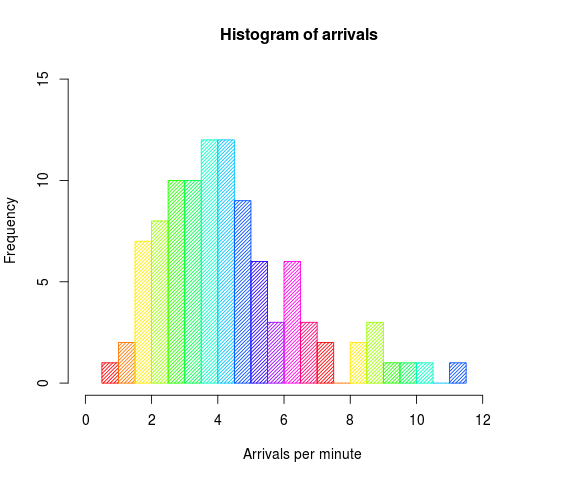
\includegraphics[scale=0.5]{12-histogram.png}
	}{Пример гистограммы.}
\end{figure}

Пример таблицы:
\begin{table}[htb]
	\centering
	\begin{tabular}{|c|c|c|c|}
		\hline
		& \dots & $\Delta_i$  & \dots \\
		\hline
		Н & \dots & $n_i$ & \dots \\
		\hline
		О & \dots & $n \, p_i$ & \dots \\
		\hline
	\end{tabular}
\end{table}